\documentclass[superscriptaddress,aps,prb,11pt]{revtex4-1}

\usepackage{amsmath}
\usepackage{graphicx}
\usepackage{color}
\usepackage{subfigure}
\usepackage{hyperref}

\begin{document}

\title{Experimental Search for Lorentz Violation in Antihydrogen}
\author{F. Isono}
\affiliation{Department of Physics, University of California, Berkeley, CA 94720-7300, USA}
\affiliation{Department of Energy Sciences, Tokyo Institute of Technology, Yokohama, 226-8502, Japan}

\author{Z. Vendeiro}
\affiliation{Department of Physics, University of California, Berkeley, CA 94720-7300, USA}

\author{J. Fajans}
\affiliation{Department of Physics, University of California, Berkeley, CA 94720-7300, USA}
\affiliation{Lawrence Berkeley National Laboratory, Berkeley, CA 94720, USA}

\author{A. Charman}
\affiliation{Department of Physics, University of California, Berkeley, CA 94720-7300, USA}
\affiliation{Lawrence Berkeley National Laboratory, Berkeley, CA 94720, USA}

\author{M. Reinsch}
\affiliation{Department of Physics, University of California, Berkeley, CA 94720-7300, USA}
\affiliation{Lawrence Berkeley National Laboratory, Berkeley, CA 94720, USA}

\author{J. S. Wurtele}
\affiliation{Department of Physics, University of California, Berkeley, CA 94720-7300, USA}
\affiliation{Lawrence Berkeley National Laboratory, Berkeley, CA 94720, USA}

\author{A. Lotta-Folks}
\affiliation{Department of Physics, University of California, Berkeley, CA 94720-7300, USA}
\affiliation{Lawrence Berkeley National Laboratory, Berkeley, CA 94720, USA}

\begin{abstract}
The advent of precision measurements on antihydrogen has opened new doors for tests of fundamental physics in the antimatter sector.  This paper retrospectively analyzes data on locations of antihydrogen annihilations in the ALPHA trap in a search for temporal variation of its charge, which would constitute a violation of Lorentz Invariance.
\end{abstract}

\maketitle

\section{}
General relativity purports that a particle's charge is independent of the observer's reference frame.  Although the theoretical underpinnings of this prediction are strong, the possibility of the small violations has been suggested by attempts to construct GUTs. In particular, Alan Kostelecky et al., first proposed spontaneous Lorentz violation in string theory \cite{kostelecky1989spontaneous} and later suggested Standard Model Extension parameters to add Lorentz-violating terms to the Standard Model \cite{colladay1998lorentz}. Experimental verification of fundamental predictions of physics are critical to assessing the axioms necessary to test the theory.  In this spirit, recent research has been performed in the hunt for Lorentz violation\cite{kostelecky2011data}. However, no measurements has proved it conclusively yet. In the antimatter sector, the ALPHA collaboration has succeeded in measuring the antihydrogen charge with high precision\cite{amol:14a}, which has opened new avenues for using antihydrogen as a tool for testing underlying physical principles.  Here, we have performed a retrospective analysis on the data collected from the ALPHA experiment in 2010 and 2011 to examine it for indications of a varying antihydrogen charge as the trap moves through space.

Over 386 antihydrogens in 320 experimental trapping attempts passed all detection criteria, hereafter referred to as cuts\cite{amol:14a}.  Only the antihydrogens that passed the cuts are included in the analysis.  The times of these detection events were distributed over 405 days and over all hours of the day (see Fig.\ref{fig:experimental_t_distributions}).  This is significant for the analysis as violations would likely be correlated with the velocity and/or orientation of the trap with respect to cosmic microwave background (CMB), which is the most likely candidate for a preferred reference frame. With this in mind, we search for an antihydrogen charge oscillation with a period of one year or one sidereal day. Orbital data was calculated using AEPHEM\cite{aephem}, an astronomical ephemeris and reduction library.

The full data set for this analysis consists of the times and $z$-positions (along trap axis) of antihydrogen annihilations after ALPHA's confining magnetic trap is quenched.  During the trapping run, a series of axial electric fields called kicks are sequentially applied to the trap to drive unbound antiprotons out and leave only antihydrogen behind. If the antihydrogen atoms have a nonzero charge, their trajectories will be perturbed by these fields and the distribution of their annihilations will be shifted.  This behavior was used to place a bound on a static antihydrogen charge in a previous publication \citep{amol:14a}.  If the charge is in fact time-dependent and periodic, then the mean annihilation position will oscillate.  The Fourier coefficients of the annihilation positions as a function of time are measured experimentally.  Simulations are then performed to determine the expected distribution of these Fourier coefficients for charge oscillations of various magnitudes at frequencies of interest.  Comparisons of the experimental value to these simulated distributions then allow bounds to be placed on the magnitude of the charge oscillation.
\\

\noindent
(RESULTS)
\\

We note that our method for setting a bound of Lorentz invariance can be done better with more precise technique to limit the error of antihydrogens' annihilation position, and with the increase of trapping rate of antihydrogens. This work provides a new big step toward the test of fundamental physics, based on the measurement of the charge of an antihydrogen.

\begin{figure}
  \subfigure[\ Event Dates]{
  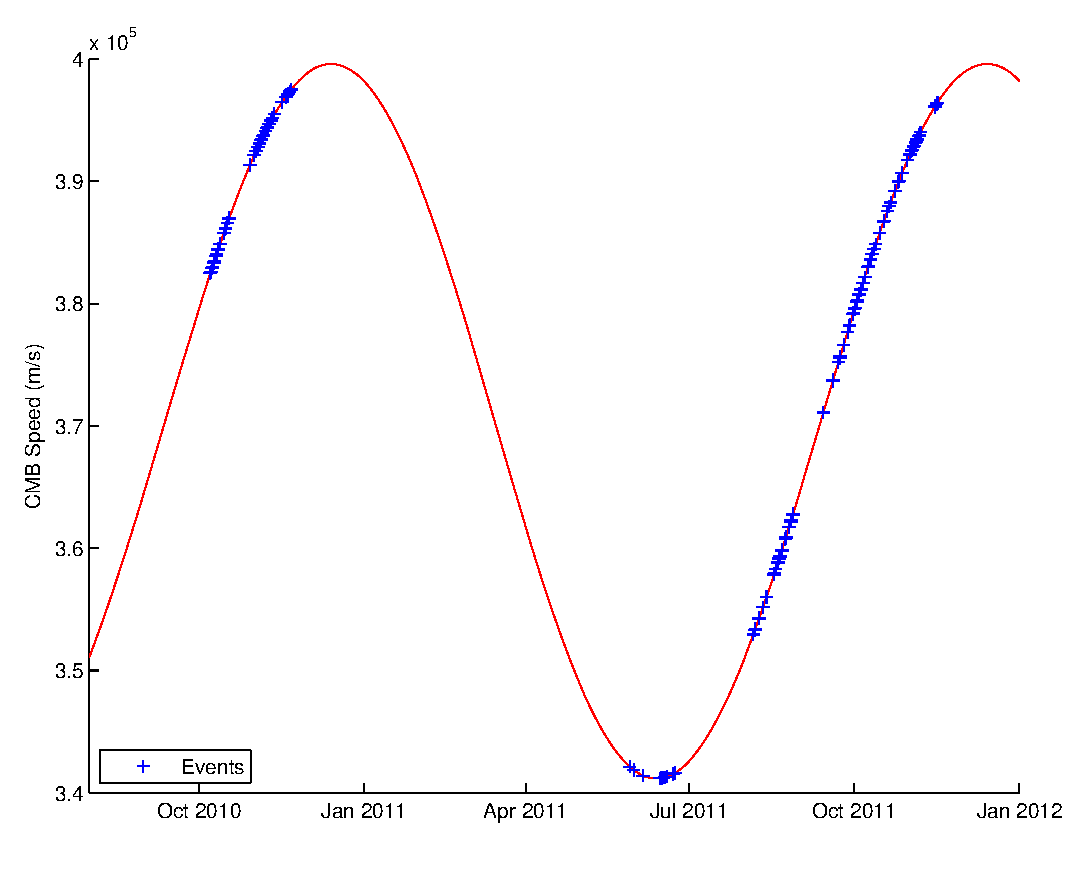
\includegraphics[scale=0.35]{True_Event_Distribution.eps}
  \label{fig:true_event_distribution}
  }
  \subfigure[\ Event Times]{
  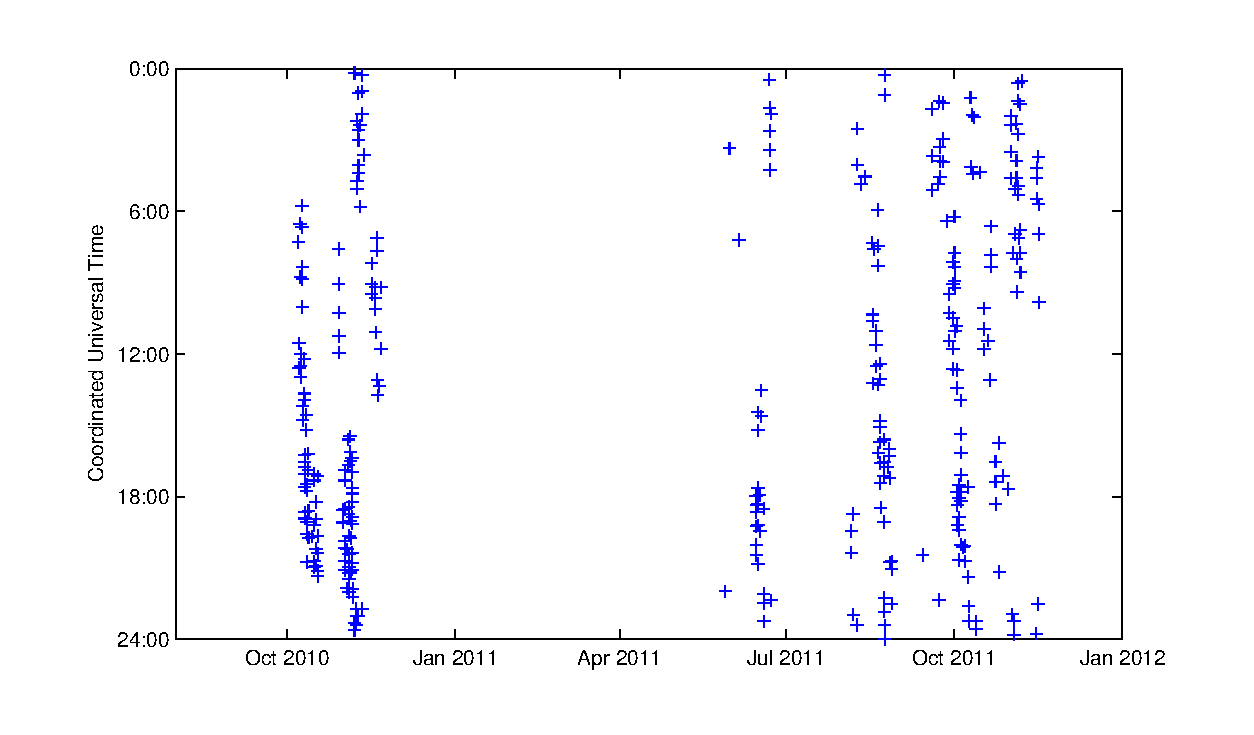
\includegraphics[scale=0.35]{eventTime_date_experiment.eps}
  \label{fig:eventTime_date_experiment}}
  \caption{\subref{fig:true_event_distribution}: The CMB speed of the Earth with the dates of $\bar{H}$ annihilation events marked.  \subref{fig:eventTime_date_experiment}: The times of day of the antihydrogen events (times are in Coordinated Universal Time).
  }
  \label{fig:experimental_t_distributions}
\end{figure}

\section{Methods Summary}
A bound on the temporal variation of the antihydrogen charge is performed by comparison of a test statistic $S$, constructed to approximate the magnitude of a Fourier coefficient, between the collected data and simulated distributions of this statistic.  A statistically significant nonzero value of $S$ would indicate a violation of Lorentz Invariance.

The full data set consists of the annihilation times and $z$-values (position along trap axis) from ALPHA's trapping attempts.  Define $f(t)$ to be a function that maps times of $\bar{H}$ annihilations to the $z$ position of those annihilations.  To be continued \ldots

\subsection*{Time Selection}
 The annihilation time of events for simulation was randomly selected from the time span when we were able to operate trapping trials, which were chosen based on the statistical data analysis of $\sim 1900$  trapping trials operated in 2010 and 2011.

 The trial time spans were assumed to be from when the first trial trap started to when the last one started within the fixed  4 $\sim$ 17 hours of time shift when we can access to Antiproton Decelerator. The first and last trial trap time were predicted by Poisson process since the former time relative to when the shift starts, and the latter time relative to when the shift ends show exponential distribution. The distributions of these two kinds of simulated time are shown in Fig.\ref{fig:time_distribution} with experimental data overlaid. Then the operation time of 320 $\pm$ 18 trapping trials succeeded in trapping $\bar{H}$ annihilation(s) were randomly selected within the time span. The time duration of the trapping trial was fixed to 10.00 minutes based on the experiment. The number of annihilation events for each successful trapping trial were chosen from the fact that the probability of getting one event per a trapping trial predicted by Poisson statistics was $\lambda=0.387532$. Note that mili seconds of time difference between more than one $\bar{H}$ annihilations in a same trapping trial were ignored since we have time information of annihilation events in order of a second. The example of time selection with this method is shown in Fig.\ref{fig:eventTime_date_sim}.

\begin{figure}
\centering
  \subfigure[\ Time from when the first trial trap was operated to when the first shift started]{
  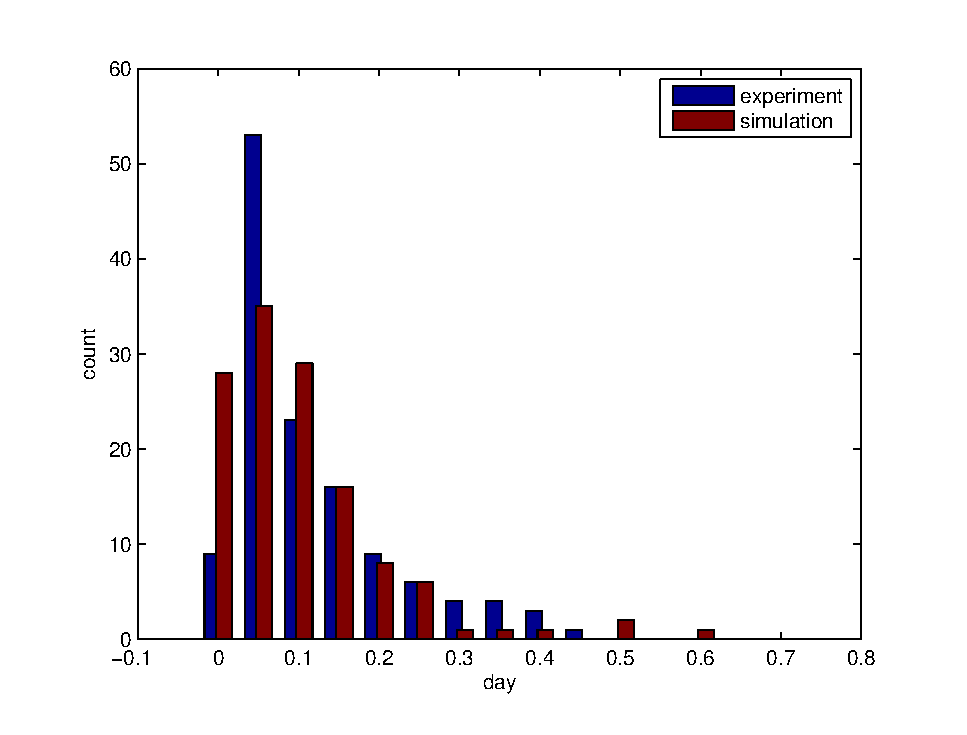
\includegraphics[scale=0.5]{startTime_distribution.eps}}
  \subfigure[\ Time from when the last shift started to when the last trial trap was operated.]{
  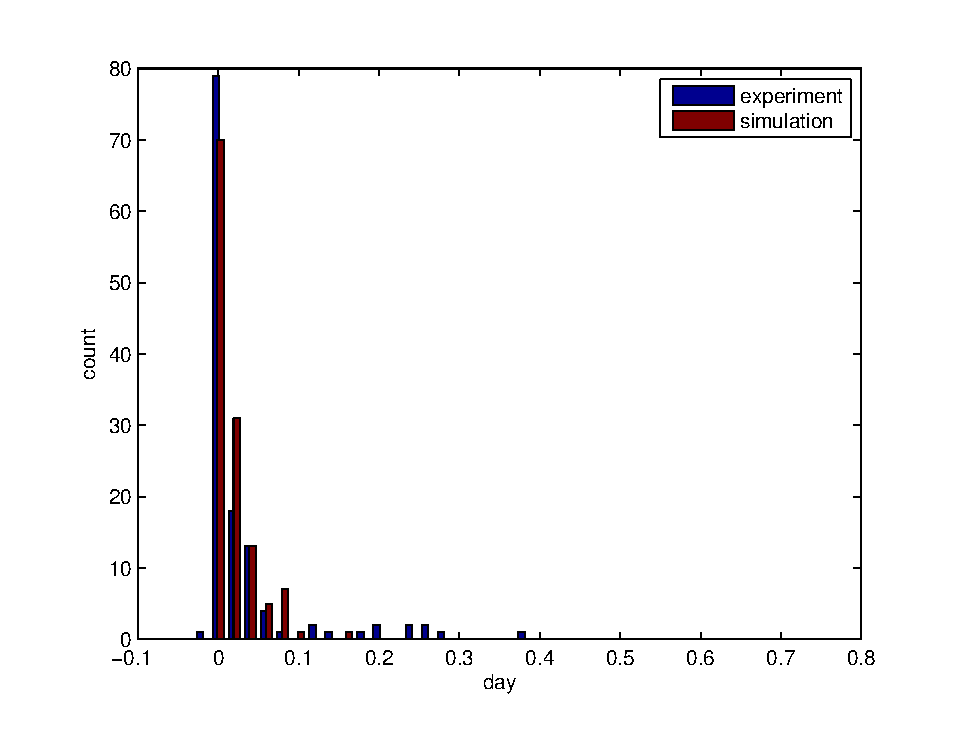
\includegraphics[scale=0.5]{endTime_distribution.eps}}
  \caption{ Distributions of simulated time spans overlaid with the experimental data. }
  \label{fig:time_distribution}
\end{figure}
 
\begin{figure}
\centering
  \subfigure[\ Experimental data]{
  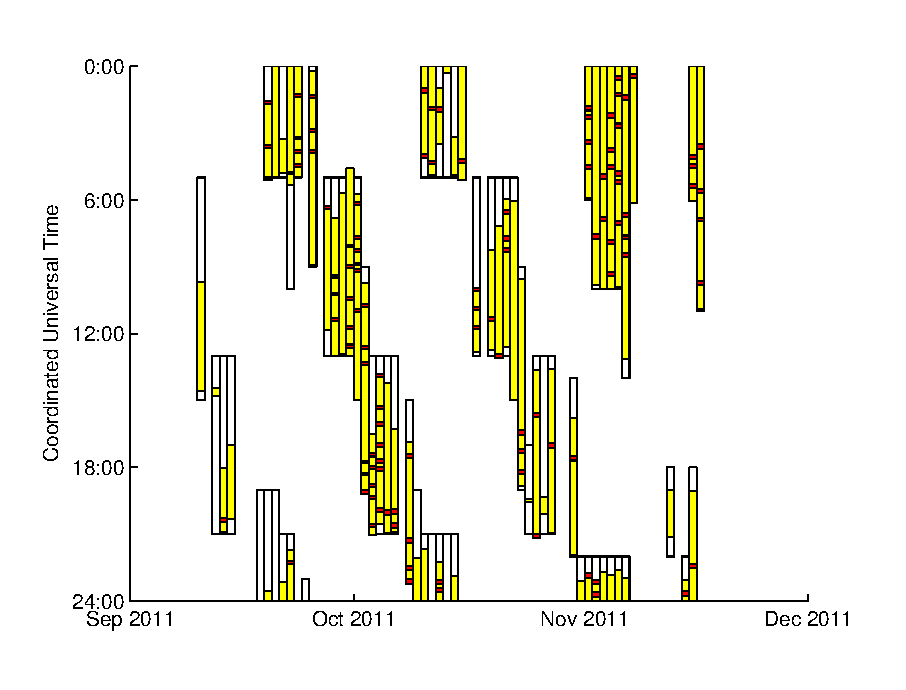
\includegraphics[scale=0.5]{eventTimeTable_experiment_example.eps}}
  \subfigure[\ Example time selection]{
  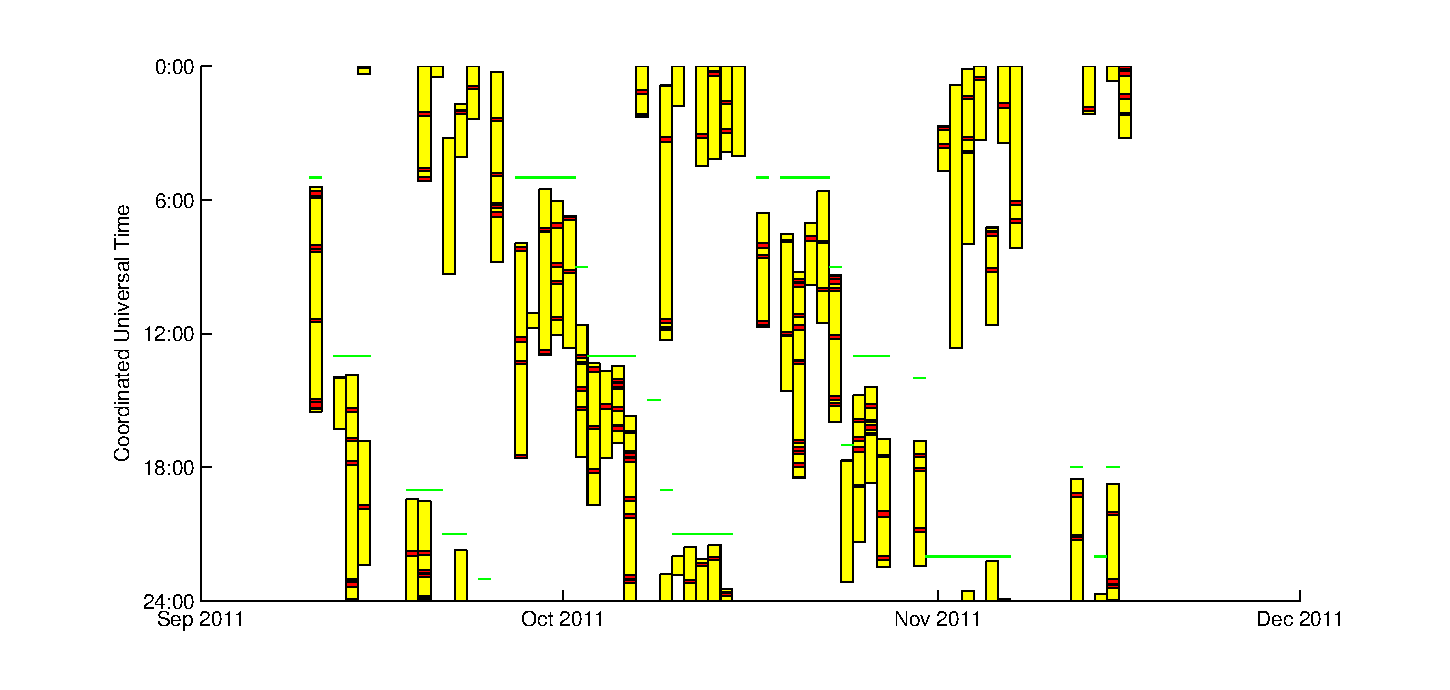
\includegraphics[scale=0.5]{eventTime_sim_example.eps}}
  \caption{The time table of (a) the experimental data and (b) example time selection in Coordinated Universal Time against day. The time span when we were able to run trapping trials (yellow boxes) was chosen within each assigned shift schedule (white boxes). Then within the trial time span, the time of 320$\pm$18 successful trapping trials (red boxes) were randomly chosen. We detected at least one annihilation event at the end of successful trapping trials (the bottom of red boxes).}
  \label{fig:eventTime_date_sim}
\end{figure}


\subsection*{Position Selection}
Creation of pseudo-data sets requires an algorithm capable of generating $z$ positions of $\bar{H}$ annihilations for arbitrary charge values.  This is achieved by randomly sampling an approximated inverse CDF of the annihilation locations along the trap axis for the given charge.

Using the symplectic integrator discussed in Ref. \onlinecite{amol:14a}, a list of annihilation $z$ coordinates is created for both quip directions for several different charges $\{q_i\}$, indexed in order of increasing charge.  These lists are then adjusted to account for effects from detector smearing and missed detections due to cosmic ray filtering criteria, also discussed in Ref. \onlinecite{amol:14a}.  For each charge $q_i$, let $D_{q_i}(z)$ denote the linear interpolation of the distribution's normalized CDF for a given direction (either left or right).  Two $D_{q_i}(z)$ are depicted in Fig. \ref{fig:z_interpolation} (blue solid lines).  Furthermore, let $D^{-1}_{q_i}(r)$ denote the inverse of $D_{q_i}(z)$.  For any one of the $q_i$, a random annihilation position $z_0$ is chosen by selecting a random value $r_0$ in the interval $(0,1)$, then setting $z_0=D^{-1}_{q_i}(r_0)$.

For a charge $q$ between the discrete $q_i$, let $q_k$ denote the $q_i$ with the largest value less than $q$.  Then $q_{k+1}$ will be the $q_i$ with the least value greater than $q$.  A random annihilation position for this $q$ is chosen by first selecting a random value $r_0$ in the interval $(0,1)$ as before, then calculating $z_0$ from Eqn. \ref{eqn:q_interpolation}.  The weights $(q_{k+1}-q)$ and $(q-q_k)$ are chosen to provide a linear interpolation between the two inverse CDFs.  The process is summarized in Fig. \ref{fig:z_interpolation}.

\begin{equation}
z_0=\frac{D^{-1}_{q_k}(r_0)*(q_{k+1}-q) +
 D^{-1}_{q_{k+1}}(r_0)*(q-q_k)}{q_{k+1}-q_k}
\label{eqn:q_interpolation}
\end{equation}

\begin{figure}
  \centering
  \subfigure[\ Full Domain of CDF]{
  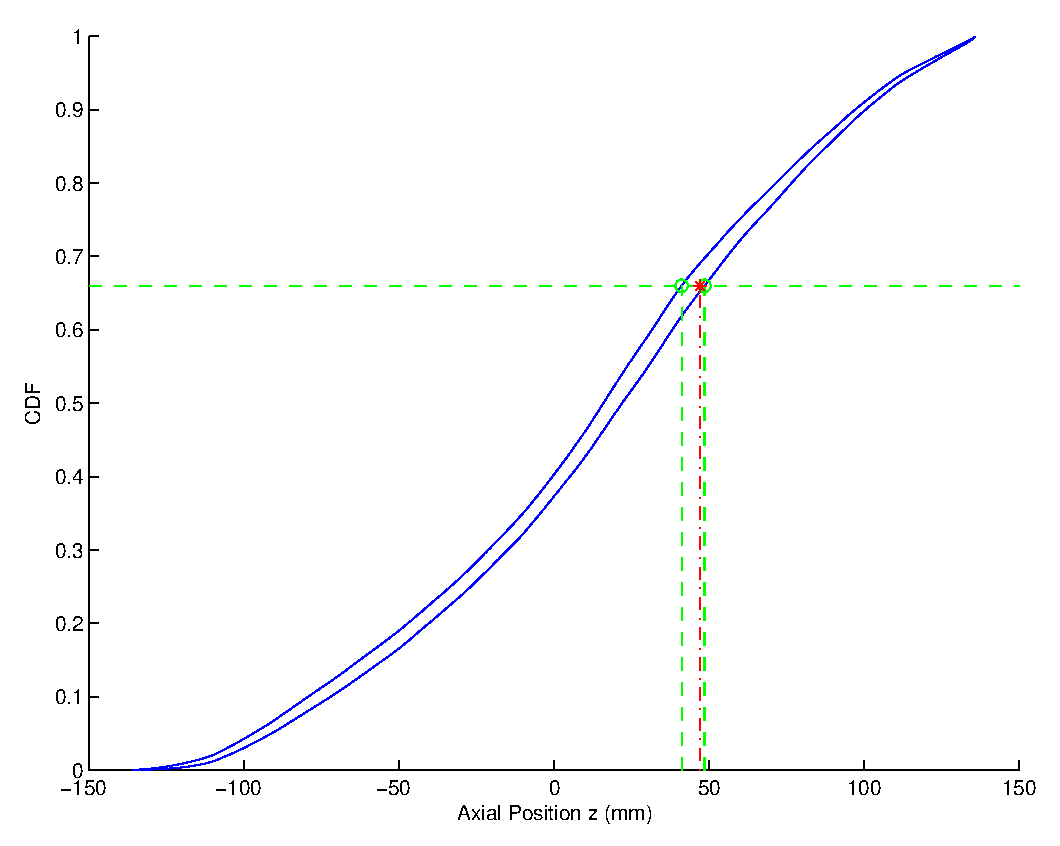
\includegraphics[scale=0.3]{CDF_Interpolation_Plot1.eps}}
  \subfigure[\ Region of Interest]{
  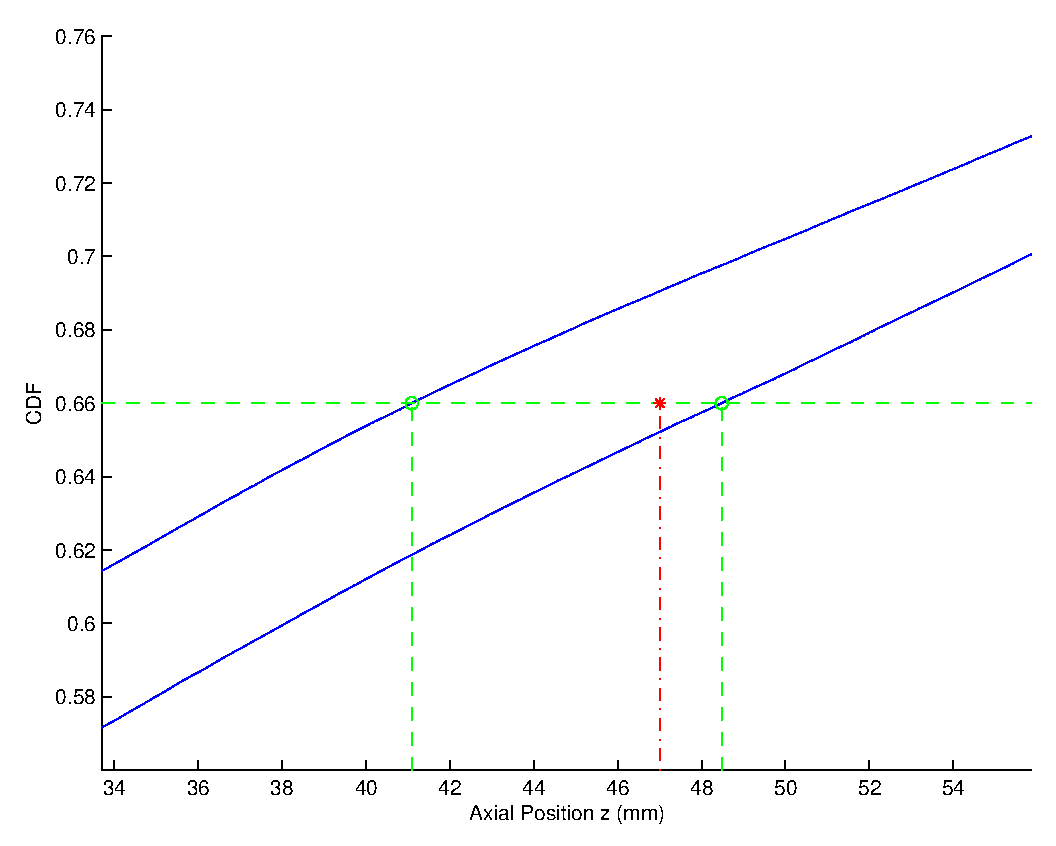
\includegraphics[scale=0.3]{CDF_Interpolation_Plot2.eps}}
  \caption{Graphical depiction of the annihilation $z$ value selection algorithm.  Empirical CDFs are generated for several different charges $q_i$ and then linearly interpolated to give $D_{q_i}(z)$.  Two such $D_{q_i}(z)$ are shown (blue solid curves).  When a $z$ position is desired for a given charge $q$, a random value $r_0$, here shown as 0.66, is picked and the values of the inverse CDFs $D^{-1}_{q_i}(r_0)$, which can be read off of the $x$-axis here, are determined (green dashed lines).  The weighted average is then taken to give the sampled $z$ value for $q$ (red dash-dot line).  Here $q$ is closer in value to $q_{k+1}$ than $q_k$.}
  \label{fig:z_interpolation}
\end{figure}

\begin{acknowledgments}
To be continued\ldots
\end{acknowledgments}

\section{Notes}
The graphs right now are created in Matlab.  In the future we may make them in Origin, which might help them look prettier.

Look for other papers on charge invariance

Mention this method can be done better in the future

\bibliographystyle{ieeetr}
\bibliography{References,bib}


\end{document}
